\chapter{Funktionsprinzip des globalen Planers}
Wie bereits erwähnt, wird die Navigationsaufgabe mithilfe zweier sukzessiver Planungsalgorithmen gelöst. Im ersten Schritt berechnet ein globaler Planer einen Weg zwischen der Ausgangs- und Zielposition, wofür die vorgegebene Karte herangezogen wird. Als Planungsalgorithmus werden im Navigation-Stack entweder Dijkstra- oder der A*-Algorithmus verwendet, die an dieser Stelle näher untersucht werden. Prinzipiell besteht die Aufgabe darin, einen Weg und Trajektorie zu ermitteln, die den Ausgangszustand des Roboters mit dem gewünschten Endzustand verbinden. Bei den gesuchten Pfaden handelt es sich um zeit- und ortskontinuierliche Kurven, woraus ein kontinuierlicher Raum von Lösungen resultiert, der nach einer optimalen durchsucht werden muss. Die Kontinuität des Suchraums stellt auf der Planungsseite eine immense Herausforderung dar, da in diesem Fall Gütefunktionale optimiert werden müssen. Um dieser Komplexität Herr zu werden, wird der Suchraum diskretisiert und die Planungsaufgabe auf die Bestimmung einer Positionsfolge reduziert.

Allerdings wird die Diskretisierung des Raumes von mehr als einer reinen Vereinfachung des Suchproblems motiviert: Der globale Planer übernimmt lediglich den ersten Schritt bei der Berechnung der letztendlichen Trajektorie. Der lokale Planer ermittelt anhand der globalen Sollkurve eine lokale Trajektorie, die in Form von Stellgrößen realisiert wird. Dabei werden neben der globalen Ortskurve auch aktuelle Sensor- und Lokalisierungsinformationen miteinbezogen, welche unter Umständen dazu führen können, dass der Roboter von der global geplanten Kurve abweicht. Insofern ergibt es wenig Sinn, bei der globalen Planung Ressourcen in eine unnötig genaue Trajektorie zu investieren; besonders dann, wenn noch nicht alle nötigen Informationen vorliegen. Für den Anfang genügt ein ungenauer, fehlerbehafteter Pfad, der die Anfangs- und Zielposition verbindet, wofür eine diskrete Darstellung des Suchraums vollkommen genügt. Des Weiteren stimmt die Forderung nach einer diskreten Darstellung des Suchraums mit den üblichen Darstellungsformen von metrischen Karten überein, denn diese repräsentieren die Umgebung in Form von diskreten Zellen.

\pdfcomment{Formulierung}Im Rahmen dieser Überlegung werden die vereinfachten Bedingungen zunächst in einer mathematischen Darstellung formuliert. Es wird angenommen, dass der Roboter in einer planen Umgebung manövriert, welche mittels einer zweidimensionalen Karte dargestellt werden kann. Hierfür wird eine metrische Karte verwendet, die den Raum in quadratische Zellen fixer Größe unterteilt. Die Positionen von Objekten innerhalb der Karten werden mithilfe des X- und Y-Indexes angegeben, wodurch die Positionsangaben von der Zellengröße entkoppelt werden. An dieser Stelle kann entweder ein deterministisches oder stochastisches Modell verwendet werden. Bei Erstem wird die Karte als Menge
\begin{equation}
M = \left\{m_{ij}\right\} \hspace{3.cm} m_{ij} \in \left\{0, 1\right\}
\end{equation}
dargestellt, wobei jede Zelle $m_{ij}$ im belegten Fall den Wert $1$ und ansonsten den Wert $0$ annimmt. Bei den so genannten Occupancy-Grids handelt es sich eine stochastische Repräsentation: Für jede Zelle wird die Wahrscheinlichkeit angegeben, ob diese belegt ist. 

Die Planungsaufgabe wird durch die Angabe einer Startposition $\mVec{x}_0$ und einer Zielposition $\mVec{x}_G$ definiert, wobei angenommen wird, dass sowohl $\mVec{x}_0$ als auch $\mVec{x}_G$ freie Zellen sind.
Zuletzt muss die Menge der möglichen Aktionen $U$ spezifiziert werden. Hier wird eine weitere Vereinfachung vorgenommen. Die eigentlichen Stellgrößen des Roboters sind dessen Translations- und Rotationsgeschwindigkeit, welche sich allerdings auf zeit- und ortskontinuierliche Trajektorien führen. Da lediglich ortsdiskrete Pfade berechnet werden sollen, ergibt es Sinn, diskrete Positionsänderungen als Aktionen zu definieren. Beispielsweise kann die Verrückung um eine Zelle entlang der X- und Y-Richtung zugelassen werden. Da die Positionen in Form von Zellenindizes beschrieben werden, kann die Verrückung durch die Addition eins Vektors ausgedrückt werden, woraus die Aktionsmenge
\begin{equation}\label{eq_Uset}
U = \left\{ 
\mVec{u}\idx{1} = \begin{bmatrix} 1 \\ 0 \end{bmatrix}, 
\mVec{u}\idx{2} = \begin{bmatrix} -1 \\ 0 \end{bmatrix},
\mVec{u}\idx{3} = \begin{bmatrix} 0 \\ 1 \end{bmatrix},
\mVec{u}\idx{4} = \begin{bmatrix} 0 \\ -1\end{bmatrix} \right\}
\end{equation}
resultiert. Von einem beliebigen Zustand $\mVec{x}\idx{n}$ ausgehend, kann mithilfe der Übergangsfunktion
\begin{equation}\label{eq_fxnew}
\mVec{x}\idx{n+1} = f(\mVec{x}_n, \mVec{u}) = \mVec{x}_n + \mVec{u}
\end{equation}
der durch die Aktion $\mVec{u}$ erreichte Zustand $\mVec{x}\idx{n+1}$ ermittelt werden.

\section{Forward-Search: Breiten Suche}\pdfcomment{Eventuell Seitenumbruch}
Stehen die Ausgangsposition $\mVec{x}\idx{0}$, die Zielposition $\mVec{x}\idx{G}$, die Menge der zulässigen Zustände $X$, welche durch die Karte $M$ definiert wird, und eine Aktionsmenge $U$ zur Verfügung, können erste rudimentäre Planungsalgorithmen entwickelt werden. Die Aufgabe besteht darin eine Sequenz von Aktionen oder Zuständen zu bestimmen, welche die Positionen $\mVec{x}\idx{0}$ und $\mVec{x}\idx{G}$ miteinander verbinden. Dabei spielt es keine Rolle, ob Aktionen oder wegzusammenhängende Zustände berechnet werden, da beide Darstellungsformen des Pfades ineinander überführt werden können. Als erster Ansatz für die Lösung des Planungsproblems kann die so genannte Forward-Search nach \cite[S. 28]{PlanAlgo} verfolgt werden:
\begin{lstlisting}[mathescape=true, caption={Ablauf der Forward-Search in Pseudocode},captionpos=bot]
Q.Insert($\mVec{x}\idx{0}$) and mark $\mVec{x}\idx{0}$ as visited
while Q not empty do
	$\mVec{x}\idx{n}$ = Q.GetFirst()
	if $\mVec{x}\idx{n} = \mVec{x}\idx{G}$
		return SUCCESS
	forall $\mVec{u}  \in U$
		$\mVec{x}\idx{n+1}$ not visited
			Mark $\mVec{x}\idx{n+1}$ as visited
			Q.Insert($\mVec{x}\idx{n+1}$)
return FAILURE
\end{lstlisting}
Der Algorithmus basiert auf einer Datenstruktur $Q$, deren Funktionsprinzip die Charakteristik des Suchalgorithmus maßgeblich prägt. Bei der Initialisierung des Algorithmus wird die Anfangsposition $\mVec{x}\idx{0}$ in die Datenstruktur eingefügt. Anschließend wird in einer Schleife die Struktur ausgelesen, wo zuerst geprüft wird, ob der aktuelle Zustand $\mVec{x}\idx{n}$ der gesuchten Zielposition $\mVec{x}\idx{G}$ gleicht; \pdfcomment{Formulierung?}gegebenenfalls terminiert die Suche. Wurde das Ziel noch nicht erreicht, werden alle möglichen Aktionen $\mVec{u}$ auf den aktuellen Zustand $\mVec{x}\idx{n}$ angewandt, wodurch jeweils ein neuer Zustand $\mVec{x}\idx{n+1}$ erzeugt wird. Falls der neue Zustand $\mVec{x}\idx{n+1}$ noch nicht geprüft wurde, wird er ebenfalls in die Datenstruktur $Q$ eingefügt. Dadurch wird der Suchraum der möglichen Zustände systematisch durchsucht, wobei eine mehrmalige Prüfung des gleichen Zustandes durch eine Markierung verhindert wird. Wenn die Datenstruktur $Q$ keine Elemente enthält, wurden alle möglichen Zustände geprüft; folglich kann das gewünschte Ziel nicht von der gegebenen Anfangsposition erreicht werden.

Das Funktionsprinzip der Datenstruktur $Q$ gibt die Reihenfolge vor, in der die neu erschlossenen Zustände überprüft werden, wodurch die Suchstrategie festgelegt wird. Arbeitet Q nach dem FIFO-Prinzip, wird der Suchraum zuerst in der Breite und anschließend in der Tiefe erforscht. Als Beispiel dient eine beliebige Startposition $\mVec{x}\idx{0}$ und die bereits genannte Aktionsmenge
\begin{equation}
U = \left\{ 
\mVec{u}\idx{1} = \begin{bmatrix} 1 \\ 0 \end{bmatrix}, 
\mVec{u}\idx{2} = \begin{bmatrix} -1 \\ 0 \end{bmatrix},
\mVec{u}\idx{3} = \begin{bmatrix} 0 \\ 1 \end{bmatrix},
\mVec{u}\idx{4} = \begin{bmatrix} 0 \\ -1\end{bmatrix} \right\}\tag{\ref{eq_Uset}}\,.
\end{equation}
Die folgenden Zustände ergeben sich nach
\begin{equation}
\mVec{x}\idx{n+1} = f(\mVec{x}_n, \mVec{u}) = \mVec{x}_n + \mVec{u}\tag{\ref{eq_fxnew}}\,.
\end{equation}
Folglich entspricht die Menge der am Iterationsschritt $1$ möglichen Zustände dem Abbild
\begin{equation}
X\idx{1} = f(\mVec{x}\idx{0}, U) = \left\{ \mVec{x}\idx{0}+\mVec{u} \hspace{5pt}\vert \hspace{5pt} \mVec{u} \in U \right\}\,.
\end{equation}
Analog kann die Menge der möglichen Zustände an einem beliebigen Schritt $n+1$ durch das Abbild
\begin{equation}
X\idx{n+1} = f(X\idx{n}, U)
\end{equation}
bestimmt werden.
Angenommen die Suche wird von einem beliebigen Startzustand $\mVec{x}\idx{0}$ begonnen, so wird im ersten Schleifendurchlauf das Abbild $X\idx{1}$ bestimmt und in die Datenstruktur eingefügt. Arbeitet diese nun nach dem FIFO-Prinzip, so werden in den folgenden Durchläufen die Elemente der Menge $X\idx{1}$ bearbeitet, wodurch die Menge $X\idx{2}$ berechnet und in die Datenstruktur eingefügt werden. Da die Elemente von $X\idx{2}$ aber nach denen von $X\idx{1}$ in die Schlange eingefügt werden, wird sichergestellt, dass zuerst alle Elemente von $X\idx{1}$ geprüft werden, bevor die Bearbeitung von $X\idx{2}$ stattfindet. Aus diesem Grund wird diese Suchstrategie als Breadth-First bezeichnet, da zuerst alle Möglichkeiten eines Iterationsschrittes geprüft werden, bevor die nachfolgende Iteration in Erwägung gezogen wird. Stellt man den Suchraum als Baum dar, wird die Bedeutung der Begriffe Tiefe und Breite deutlich.

\pdfcomment{Baumbild}
Mit der Breadth-First-Search liegt ein systematischer Ansatz vor, der einen Pfad zum Ziel findet, falls ein solcher existiert. Außerdem ist recht leicht ersichtlich, dass der Algorithmus immer auf einen möglichst kurzen Lösungspfad führt. Um das Konzept zu illustrieren, wird folgendes Beispiel betrachtet: Ein Roboter befindet sich in einem Korridor an einer bekannten Position $\mVec{x}\idx{0}$. Die Umgebung wurde mittels einer deterministischen Karte
\begin{equation}
M = \left\{m_{ij}\right\} \hspace{2.5cm} \forall m_{ij} \in \left\{0, 1\right\}
\end{equation}
dokumentiert, wobei die Zellen eine Kantenlänge von $25 \text{cm}$ besitzen. Die Zielposition $\mVec{x}\idx{G}$ liegt am Ende des Korridors. Das Ergebnis der Breitensuche zeigt die folgende Abbildung, an der ersichtlich wird, dass es sich um 
\pdfcomment{Hierfehlt was, wo wird das Beispie lmit gazebo erklärt?}
\begin{figure}[!ht]
\centering
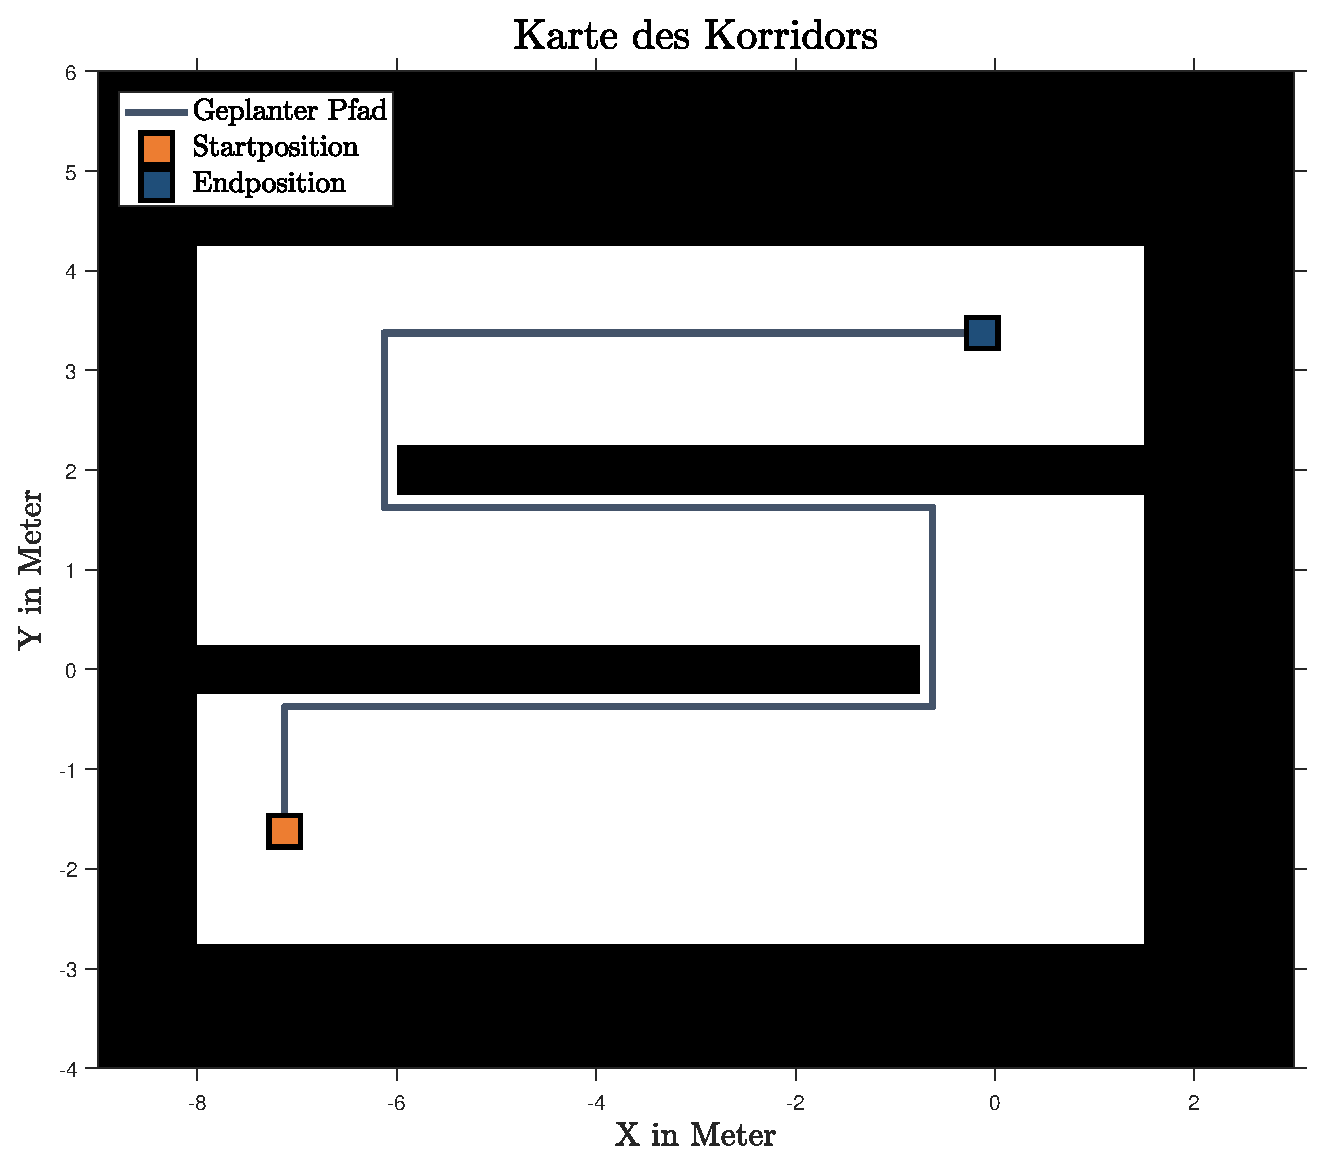
\includegraphics[width=0.7\linewidth]{img/KorridorBeispiel_img1.eps}
\caption{Ergebnis der Breitensuche}
\end{figure}


\section{Forward-Search: Tiefensuche}\pdfcomment{Seitenumbruch?}
Die komplementäre Suchstrategie wird als Depth-First-Search bezeichnet, bei der zuerst die Tiefe des Suchbaums erforscht wird, bevor parallele Zweige überprüft werden. Die Umsetzung der Depth-First-Search erfolgt indem die Datenstruktur Q als LIFO-Speicher implementiert wird. Dadurch kann im Vergleich zu der Breadth-First-Search die Suchzeit unter Umständen drastisch reduziert werden, allerdings resultieren für gewöhnlich längere Pfade. Wenn die Anzahl der Iterationsschritte oder die Menge der zulässigen Zustände begrenzt sind, wird auch die Depth-First-Search zu einem systematischen Suchansatz. Das heißt der Algorithmus stößt garantiert auf ein Ergebnis, falls ein solches existiert. Durch das LIFO-Prinzip der Datenstruktur wird das Ergebnis der zuletzt ausgeführten Aktion unmittelbar weiterverfolgt. \pdfcomment{Wiederholung dadurch}Dadurch bekommt die Reihenfolge, in der die möglichen Aktionen $\mVec{u}$ appliziert werden, eine zentrale Bedeutung, \pdfcomment{Formulierung}da dadurch die Suchrichtung vorgegeben wird. Die folgenden Abbildungen zeigen die Auswirkungen einer veränderten Aktionsreihenfolge anhand des Korridorbeispiels.

\begin{figure}[ht!]
\centering
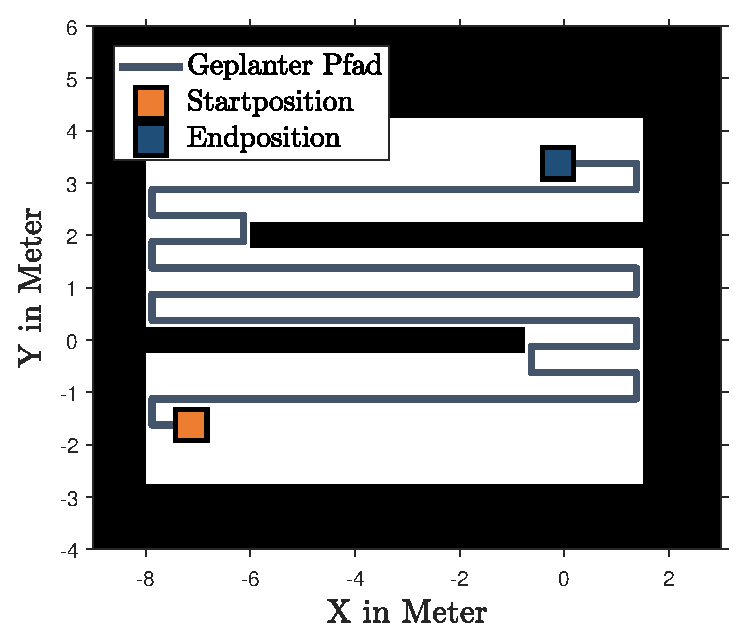
\includegraphics[width=0.45\linewidth]{img/KorridorBeispiel_img2.eps}
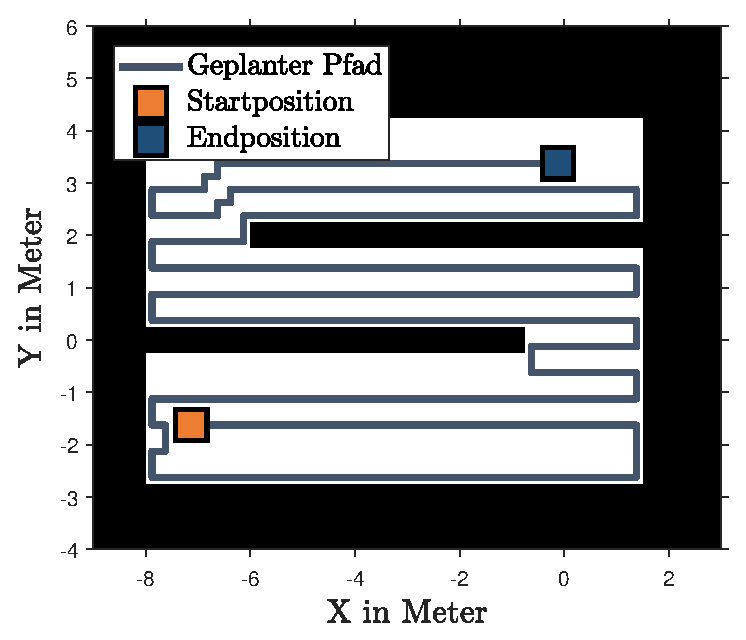
\includegraphics[width=0.45\linewidth]{img/KorridorBeispiel_img3.eps}

\vspace*{0.5cm}

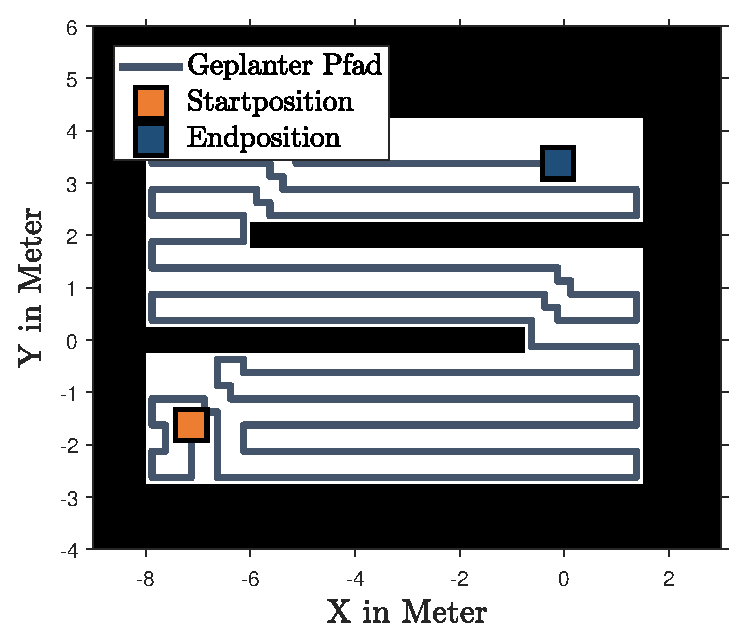
\includegraphics[width=0.45\linewidth]{img/KorridorBeispiel_img4.eps}
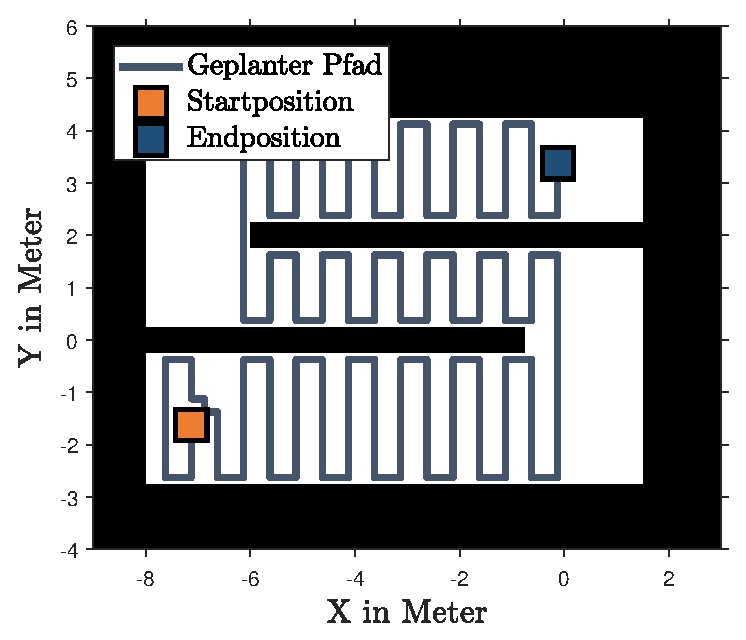
\includegraphics[width=0.45\linewidth]{img/KorridorBeispiel_img5.eps}
\caption{Ergebnisse der Tiefensuche bei unterschiedlichen Reihenfolge der Aktionen}
\end{figure}

Prinzipiell kann die Suche - unabhängig von der gewählten Strategie - auch von der Zielposition ausgehend beginnen. In diesem Fall wird von einer so genannten Backwards-Search gesprochen. Werden Forward- und Backward-Search simultan verfolgt, resultiert die so genannten Bidirectional-Search. Diese Adaptionen können unter Umständen verkürzte Suchzeiten liefern, werden an dieser Stelle aber nicht weiterverfolgt, da dieser Aspekt bei dem hiesigen Anwendungsfall nicht zum Tragen kommt.

\section{Optimale Suche und Planung}\pdfcomment{Idiotenapostroph und so}
In den bisherigen Suchalgorithmen bestand die Aufgabe lediglich darin,\pdfcomment{Alternativen für bestand darin} eine Pfad zwischen Ausgangs- und Zielposition zu finden. Dies hatte unter anderem zur Folge, dass starke Unterschiede zwischen den Lösungen der verschiedenen Ansätze resultierten. Besonders bei der Depth-First-Search kamen zum Teil äußerst umständliche Pfade zu Stande. Aus diesem Grund soll im nächsten Schritt eine Bewertung der Lösungsmöglichkeiten eingeführt werden, die genutzt wird, um einen optimalen Pfad im Sinne dieses Gütekriteriums zu ermitteln. Bei der globalen Pfadplanung sollen prinzipiell zwei Aspekte beachtet werden: Einerseits soll der resultierende Pfad möglichst kurz sein, andererseits soll ein gewisser Abstand zu belegten Zellen der Karte gehalten werden bzw. die belegten Zellen sollen von dem Pfad nicht durchkreuzt werden. Um diese Vorgaben in einem Gütekriterium auszudrücken, wird die Karte in eine sogenannte Kostenkarte transformiert. Diese ordnet jeder Zelle einen Aufwand zu, wodurch es möglich wird verschiedenen Pfade zu bewerten und miteinander zu vergleichen. Die Kosten eines Pfades ergeben sich aus der Summe der enthaltenen Zellen. Ein Beispiel für eine mögliche Bewertung der Zellen ordnet jeder freien Zelle den Aufwand $1$ und jeder belegten Zelle den Wert $\infty$ zu. Durch letzteren wird sichergestellt, dass belegte Zellen vermieden werden. Die Gewichtung von freien Zellen führt dazu, dass kürzere Pfade mit geringeren Kosten verbunden sind. Eine Möglichkeit, um einen im Kontext der Kostenkarte optimalen Pfad zu berechnen, stellt Dijkstra's Algorithmus dar. Dieser gleicht im Grundprinzip den bisher betrachteten Vorgehensweise, mit dem Unterschied, dass die Datenstruktur $Q$ so sortiert wird, dass das Element mit den aktuell geringstem Kostenaufwand am Anfang der Liste steht. Zusätzlich muss in dem Fall, dass ein Zustand geprüft wird, der bereits besucht worden ist, verglichen werden, welcher der beiden Pfade den geringeren Aufwand benötigt.

\begin{lstlisting}[mathescape=true, caption={Dijkstra's Algorithmus in Pseudocode}]
Q.Insert($\mVec{x}\idx{0}$) and mark $\mVec{x}\idx{0}$ as visited
while Q not empty do
	$\mVec{x}\idx{n}$ = Q.GetFirst()
	if $\mVec{x}\idx{n} = \mVec{x}\idx{G}$
		return SUCCESS
	forall $\mVec{u}  \in U$
		if $\mVec{x}\idx{n+1}$ not visited
			Mark $\mVec{x}\idx{n+1}$ as visited
			Q.Insert($\mVec{x}\idx{n+1}$)
		else
			resolve duplicate
return FAILURE
\end{lstlisting}
Die folgende Abbildung zeigt die Ergebnisse der Suche bei dem bekannten Anwendungsbeispiel.
\begin{figure}[ht!]
\centering
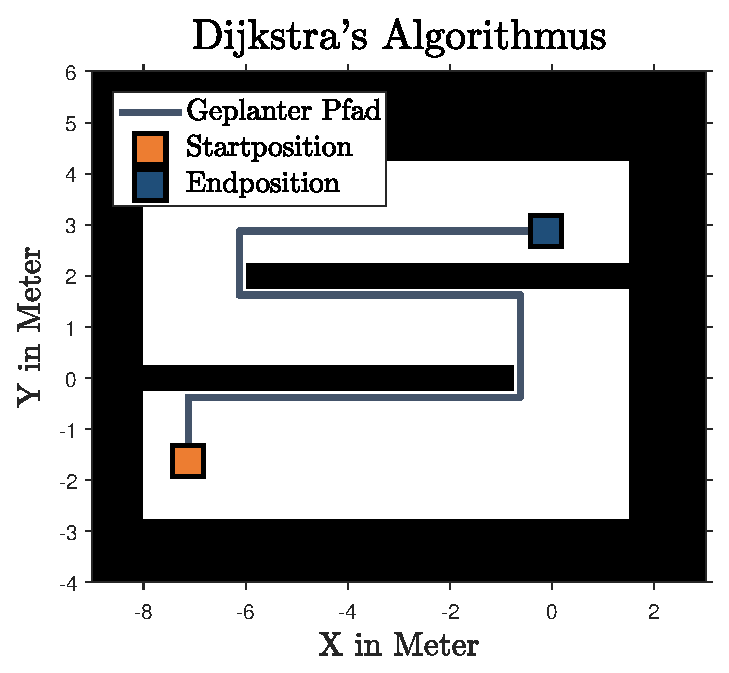
\includegraphics[width=0.5\linewidth]{img/KorridorBeispiel_img6.eps}
\caption{Ergebnis mit Dijkstra's Algorithmus}
\end{figure}

\subsection{A*}
Indem bei Dijakstra's Algorithmus die Liste $Q$ nach aufsteigenden Kosten sortiert wird, kann gesichert werden, dass die Suche zu einem optimalen Ergebnis führt. Allerdings bringt dieses Vorgehen einen zum Teil unnötigen Suchaufwand mit sich, was recht leicht illustriert werden kann: Um möglichst kurze Pfade zu erhalten, wurde jeder weitere Schritt mit einem fixen Aufwand bewertet. Dies hat zur Folge, dass die kürzesten Pläne an den Anfang der Liste rücken, inklusive der Pfade, die entweder zu kurz sind, um das Ziel überhaupt erreichen zu können, \pdfcomment{Formulierung}als auch solche die sich in eine falsche Richtung bewegen. Insofern erzwingt die sortierte Datenstruktur eine Breitensuche, da kurze Pfade fälschlicherweise - zumindest teilweise fälschlicherweise - mit weniger Aufwand verbunden sind.

Ein Ansatz, um dieser Problematik vorzubeugen, stellt der $A*$ Algorithmus dar, der nach dem identischen Grundprinzip wie Dijakstra's Algorithmus arbeitet. Lediglich das Gewichtungskonzept der Pläne unterscheiden die beiden Vorgehensweisen. Für jede Position $\mVec{x}\idx{n}$ existiert ein optimaler Pfad, welcher $\mVec{x}\idx{n}$ mit der Zielposition $\mVec{x}\idx{G}$ verbindet. Die Kosten des optimalen Pfades werden von der Funktion $G^*(\mVec{x}\idx{n})$ beschrieben\pdfcomment{Der Satz ist bisschen fehl am Platz}. Die Idee des $A*$ Algorithmus besteht darin, neben den Kosten des Pfades von $\mVec{x}\idx{0}$ zu $\mVec{x}\idx{n}$ auch die verbleibenden Kosten nach $\mVec{x}\idx{G}$ zu beachten. Dadurch werden kürzere Pfade nicht mehr aus Prinzip bevorzugt, sondern lediglich dann, wen ihre erwarteten Kosten bis zum Ziel ebenfalls gering sind. Da die optimalen Kosten $G^*(\mVec{x}\idx{n})$ nicht bekannt sind müssen sie approximiert werden, wofür eine heuristische Schätzung $G(\mVec{x}\idx{n})$ eingeführt wird. An die Heuristik ist die Beindung geknöpft, dass die geschätzten Kosten $G(\mVec{x}\idx{n})$ stets kleiner oder gleich der optimalen Kosten $G^*(\mVec{x}\idx{n})$ sind:
\begin{equation}
G(\mVec{x}\idx{n}) \leq G^*(\mVec{x}\idx{n}) \hspace{2.5cm} \forall \mVec{x}\idx{n} \in X\,.
\end{equation}
Als Beispiel wird wieder die Navigation durch den Korridor betrachtet. Hier wurde jede Verrückung mit dem Aufwand $1$ gewichtet, woraus folgt, dass die Kosten zwischen $\mVec{x}\idx{n}$ und $\mVec{x}\idx{G}$ mindestens gleich der absoluten Differenzen zwischen den X- und Y-Koordinaten der beiden Positionen sein muss. Im Falle, dass ein Hindernis den direkten Weg zwischen $\mVec{x}\idx{n}$ und $\mVec{x}\idx{G}$ versperrt nehmen die optimalen Kosten $G^*(\mVec{x}\idx{n})$ weiter zu, weshalb
\begin{equation}
G(\mVec{x}\idx{n}) = \vert x\idx{n} - x\idx{G}\vert + \vert y\idx{n} - y\idx{G}\vert \leq G^*(\mVec{x}\idx{n}) \hspace{2cm} \forall \mVec{x}\idx{n} \in X
\end{equation}
stets gilt. Somit stellt $G(\mVec{x}\idx{n})$ eine legitime Approximation der optimalen Kosten $G^*(\mVec{x}\idx{G})$ dar. Wird diese Forderung an die Kostenschätzung eingehalten, kann bewiesen werden, dass der $A*$ Algorithmus stets eine optimale Lösungs findet, insofern diese existiert \cite[S. 32]{PlanAlgo}\cite{SecRef1,SecRef2}. Bei der - recht konservativen - Schätzung $G(\mVec{x}\idx{n})=0$ geht das $A*$ Verfahren in Dijkstra's Algorithmus über.
\begin{figure}[ht!]
\centering
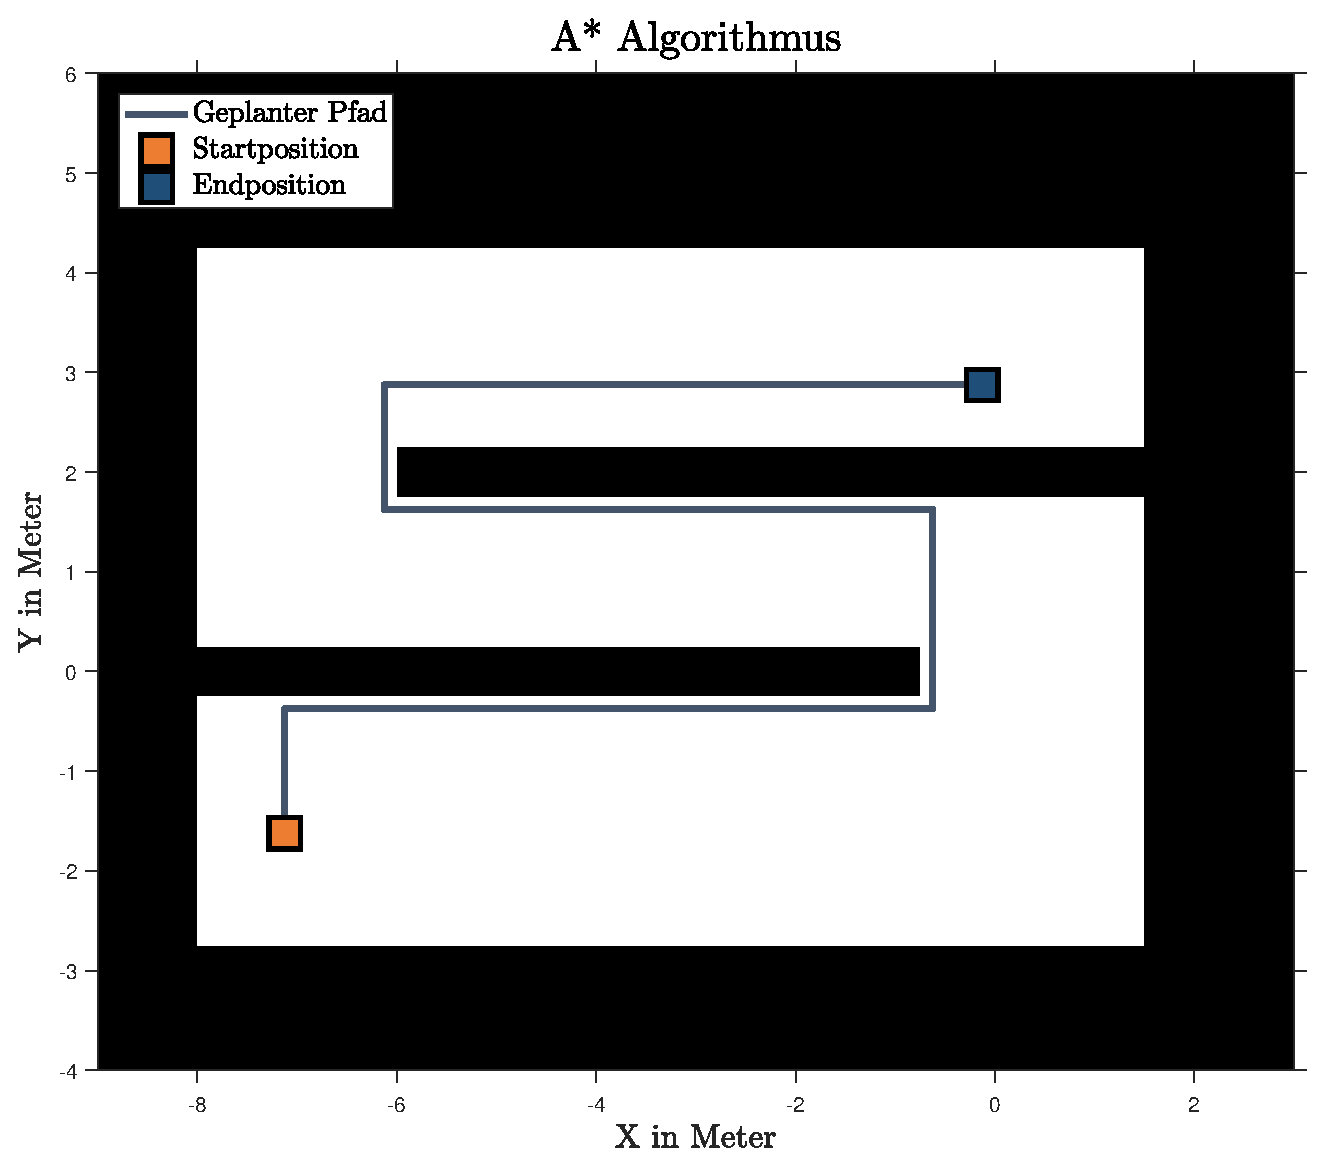
\includegraphics[width=0.5\linewidth]{img/KorridorBeispiel_img7.eps}
\caption{Ergebnis mit dem A* Algorithmus}
\end{figure}